\chapter{Edici\'{o}n B\'{a}sica}
\chaptertoc 
\begin{objetivos}
\begin{lista}
\item Comprender el esquema básico de funcionamiento de \TeX\, y \LaTeX .
\item Conocer las diferentes salidas que produce \LaTeX.
\item Conocer las diferentes herramientas que intecactuan con \LaTeX.
\item Aprender a instalar \LaTeX\, en diferentes sistemas.
\end{lista}
\end{objetivos}
\section{Introducción}

A diferencia de un procesador de textos como Writer, con \LaTeX{}
tenemos un control más adecuado sobre cualquier aspecto tipográfico
del documento. 

\LaTeX{} formatea las páginas de acuerdo a la clase de documento especificado
por el comando \lstinline+\documentclass{}+, por ejemplo, \lstinline+\documentclass{report}+
formatea el documento de tal forma que el producto es un documento
con formato de artículo. 

Un documento \LaTeX{} puede tener texto ordinario junto con texto
en modo matemático. Los comandos vienen precedidos por el símbolo
“\lstinline+\+ ” (barra invertida).

Hay comandos que funcionan en modo texto y hay comandos que solo funcionan
en modo matemático, pero para escribir en modo matemático hay varios
entornos el más común es el entorno delimitado por dos signos de dólar
(\lstinline+$...$+) .
\section{Ordenes en  \TeX\, y  \LaTeX:}

\begin{description}
\item[$\blacksquare$] Comienzan por una barra invertida: 
(( $\backslash$))

\item[$\blacksquare$] Distinguen may\'{u}sculas y min\'{u}sculas

\item[$\blacksquare$] $\ $Dos tipos:
\end{description}

1. con letras s\'{o}lo (pueden ser varias)

2. con car\'{a}cter especial (uno s\'{o}lo)

\begin{description}
\item[$\blacksquare$]  \TeX \, ignora los espacios en blanco justo despu\'{e}s de
un mandato: para tenerlos en cuenta, escribir \lstinline+\,+

\item[$\blacksquare$] Par\'{a}metros: [opcionales] y \{obligatorios\}
\end{description}

\subsection{Ejemplos de comandos}

\begin{description}
\item[$\spadesuit$] Comentarios: a partir de signo \%, son ignorados
\end{description}

Veamos algunas ordenes:
\lstinline+\TeX \LaTeX      %  \\es una orden de tipo 2+\par
Como podemos observar los dos logos aparecen juntos \\
\TeX \LaTeX  \par    %  \\es una orden de tipo 2
para que se separen debemos colocar un comando de indique el espacio, por ejemplo un espacio normal\\
\lstinline+\TeX \,\LaTeX    \\[2ex] \today\\[4ex]+\par
\TeX \,\LaTeX     \\[2ex]
\today\\[4ex]

\lstinline+\textbf{texto resaltado}+\par

\textbf{texto resaltado}


\subsection{Caracteres especiales}

Los caracteres con un significado especial, si se desean transcribir hay que
indicarlo de alguna manera:
\begin{verbatim}
$ & % # _ { } ~^\
\$ \& \% \# \_ \{ \}
\\  \verb+ ~ ^ \+
\end{verbatim}




\section{Mi primer documento}
\subsection{Estructura de un fichero de entrada}

Cuando \LaTeXe{} procesa un fichero de entrada, espera de \'el que
siga una determinada \wi{estructura}. Todo fichero de entrada debe
comenzar con la orden
\begin{code}
\lstinline+\documentclass{...}+
\end{code}
Esto indica qu\'e tipo de documento es el que se pretende crear.
Tras esto, se pueden incluir \'ordenes que influir\'an sobre el
estilo del documento entero, o puede cargar \wi{paquete}s que
a~nadir\'an nuevas propiedades al sistema de \LaTeX. Para cargar
uno de estos paquetes se usar\'a la instrucci\'on
\begin{code}
\lstinline+\usepackage{...}+
\end{code}

Cuando todo el trabajo de configuraci\'on est\\'e
realizado\footnote{El
  \'area entre \texttt{\bs documentclass} y \texttt{\bs
    begin$\mathtt{\{}$document$\mathtt{\}}$} se llama
  \emph{\wi{pre\'ambulo}}.} entonces comienza el cuerpo del texto con
la instrucci\'on
\begin{code}
\lstinline|\begin{document}|
\end{code}

A partir de entonces se introducir\'a el texto mezclado con algunas
instrucciones \'utiles de \LaTeX. Al finalizar el documento debe
ponerse la orden
\begin{code}
\lstinline|\end{document}|
\end{code}
LaTeX{} ingorar\'a cualquier cosa que se ponga tras esta
instrucci\'on.

La figura~\ref{mini} muestra el contenido m\'inimo de un fichero de
\LaTeXe. En la figura~\ref{document} se expone un \wi{fichero de
  entrada} algo m\'as complejo.

\begin{example}
%\documentclass{article}
%\begin{document}
%Lo peque~no es bello.
%\end{document}
\end{example}

Ejemplo para un art\'iculo cient\'ifico en español.
\begin{problema}
\documentclass[a4paper,11pt]{article}
\usepackage{latexsym}
\usepackage[activeacute,spanish]{babel}
\author{H.~Partl}
\title{Minimizando}
\frenchspacing
\begin{document}
\maketitle \tableofcontents
\section{Inicio}
Bien\ldots{} y aqu\'i comienza
mi art\'iculo tan estupendo.
\section{Fin}
\ldots{} y aqu\'i acaba.
\end{document}
\end{problema}




\section{El formato del documento}

\subsection{Clases de documentos}\label{sec:documentclass}

Cuando procesa un fichero de entrada, lo primero que necesita
saber \LaTeX{} es el tipo de documento que el autor quiere crear.
Esto se indica con la instrucci\'on \ci{documentclass}.
\begin{command}
\ci{documentclass}\ \lstinline+{opciones}{clase}+
\end{command}
\noindent En este caso, la \emph{clase} indica el tipo de
documento que se crear\'a. En la tabla~\ref{documentclasses} se
muestran las clases de documento que se explican en esta
introducci\'on. La distribuci\'on de \LaTeXe{} proporciona m\'as
clases para otros documentos, como cartas y transparencias. El
par\'ametro de \emph{\wi{opciones}} personaliza el comportamiento
de la clase de documento elegida. Las opciones se deben separar
con comas. En la tabla~\ref{options} se indican las opciones m\'as
comunes de las clases de documento est\'andares.


\begin{table}[!bp]
\caption{Clases de documentos} \label{documentclasses}
\begin{description}

\item [\normalfont\texttt{article}] para art\'iculos de revistas
  especializadas, ponencias, trabajos de pr\'acticas de formaci\'on,
  trabajos de seminarios, informes peque'nos, solicitudes,
  dict\'amenes, descripciones de programas, invitaciones y muchos
  otros.\index{articulo@art\'iculo}%
\index{clase \texttt{article}@clase article}
\item [\normalfont\texttt{report}] para informes mayores que constan
  de m\'as de un cap\'itulo, proyectos fin de carrera, tesis doctorales,
  libros peque'nos, disertaciones, guiones y
  similares.\index{informe}\index{clase \texttt{report}@clase report}
\item [\normalfont\texttt{book}] para libros de
  verdad\index{libro}\index{clase \texttt{book}@clase book}
\item [\normalfont\texttt{slide}] para transparencias. Esta clase emplea
  tipos grandes \textsf{sans serif}.
  \index{transparencias}\index{clase \texttt{slide}@clase slide}
\end{description}
\end{table}

\begin{table}[!bp]
\caption{Opciones de clases de documento} \label{options}
\begin{flushleft}
\begin{description}
\item[\normalfont\texttt{10pt}, \texttt{11pt}, \texttt{12pt}] \quad
  Establecen el tama~no (cuerpo) para los tipos. Si no se especifica
  ninguna opci\'on, se toma \texttt{10pt}.\index{tama~no de los
    tipos!del documento}
\item[\normalfont\texttt{a4paper}, \texttt{letterpaper}, \ldots] \quad
  Define el tama~no del papel. Si no se indica nada, se toma
  \texttt{letterpaper}. Aparte de \\'este se puede elegir
  \texttt{a5paper}, \texttt{b5paper}, \texttt{executivepaper} y
  \texttt{legalpaper}. \index{papel legal} \index{tama~no del
    papel}\index{papel DIN-A4} \index{papel de carta} \index{papel DIN-A5}\
  \index{papel DIN-B5} \index{papel ejecutivo}

\item[\normalfont\texttt{fleqn}] \quad Dispone las ecuaciones hacia la
  izquierda en vez de centradas.

\item[\normalfont\texttt{leqno}] \quad Coloca el n\'umero de las
  ecuaciones a la izquierda en vez de a la derecha.
  \vspace{5cm}

\item[\normalfont\texttt{titlepage}, \texttt{notitlepage}] \quad
  Indica si se debe comenzar una p\'agina nueva tras el \wi{t\'itulo del
    documento} o no. Si no se indica otra cosa, la clase
  \texttt{article} no comienza una p\'agina nueva, mientras que \texttt{report}
  y \texttt{book} s\'i.\index{titlepage@\texttt{titlepage}}

\item[\normalfont\texttt{twocolumn}] \quad Le dice a \LaTeX{} que
  componga el documento en \wi{dos columnas}.

\item[\normalfont\texttt{twoside, oneside}] \quad Especifica si se
  debe generar el documento a una o a dos caras.  En caso de no
  indicarse otra cosa, las clases \texttt{article} y \texttt{report}
  son a una cara y la clase \texttt{book} es a dos.

\item[\normalfont\texttt{openright, openany}] \quad Hace que los
  cap\'itulos comienzen o bien s\'olo en p\'aginas a la derecha, o bien
  en la pr\'oxima que est\\'e disponible. Esto no funciona con la clase
  \texttt{article}, ya que en esta clase no existen cap\'itulos. De
  modo predeterminado, la clase \texttt{report} comienza los
  cap\'itulos en la pr\'oxima p\'agina disponible y la clase
  \texttt{book} las comienza en las p\'aginas a la derecha.
\end{description}
\end{flushleft}
\end{table}

Por ejemplo: un fichero de entrada para un documento de \LaTeX{}
podr\'ia comenzar con
\begin{code}
\ci{documentclass}\verb|[11pt,twoside,a4paper]{article}|
\end{code}
Esto le indica a \LaTeX{} que componga el documento como un
\emph{art\'iculo} utilizando tipos del cuerpo 11, y que produzca un
formato para impresi\'on a \emph{doble cara} en \emph{papel
DIN-A4}.

\pagebreak[2]
\subsection{Paquetes}
\index{paquete} Mientras escribe su documento, probablemente se
encontrar\'a en situaciones donde el \LaTeX{} b\'asico no basta para
solucionar su problema. Si desea incluir \wi{gr\'aficos}, \wi{texto
en
  color} o el c\'odigo fuente de un fichero, necesita mejorar las
capacidades de \LaTeX. Tales mejoras se realizan con ayuda de los
llamados \emph{paquetes.} Los paquetes se activan con la orden
\begin{command}
\ci{usepackage}\verb|[|\emph{opciones}\verb|]{|\emph{paquete}\verb|}|
\end{command}
\noindent donde \emph{paquete} es el nombre del paquete y
\emph{opciones} es una lista palabras clave que activan funciones
especiales del paquete, a las que \LaTeX{} les a~nade las opciones
que previamente se hayan indicado en la orden
\verb|\documentclass|. Algunos paquetes vienen con la
distribuci\'on b\'asica de \LaTeXe{} (v\\'ease la
tabla~\ref{packages}). Otros se proporcionan por separado. En la
\guia{} puede encontrar m\'as informaci\'on sobre los paquetes
disponibles en su instalaci\'on local. La fuente principal de
informaci\'on sobre \LaTeX{} es \companion. Contiene descripciones
de cientos de paquetes, as\'i como informaci\'on sobre c\'omo
escribir sus propias extensiones a \LaTeXe.

\begin{table}[!hbp]
\caption{Algunos paquetes distribuidos con \LaTeX}
\label{packages}
\begin{description}
\item[\normalfont\pai{doc}] Permite la documentaci\'on de paquetes y
  otros ficheros de \LaTeX.\\ Se describe en \texttt{doc.dtx} y en
  \companion.

\item[\normalfont\pai{exscale}] Proporciona versiones escaladas de
  los tipos adicionales para matem\'aticas.\\
 Descrito en \texttt{ltexscale.dtx}.

\item[\normalfont\pai{fontenc}] Especifica qu\\'e \wi{codificaci\'on de
    tipo} debe usar \LaTeX.\\ Descrito en \texttt{ltoutenc.dtx}.
    \vspace{5cm}

\item[\normalfont\pai{ifthen}] Proporciona instrucciones de la forma\\
  `si\ldots{} entonces\ldots{} si no\ldots'\\ Descrito en
  \texttt{ifthen.dtx} y en \companion.

\item[\normalfont\pai{latexsym}] Para que \LaTeX{} acceda al tipo
  de s\'imbolos, se debe usar el paquete \texttt{latexsym}.\\ Descrito
  en \texttt{latexsym.dtx} y en \companion.

\item[\normalfont\pai{makeidx}] Proporciona instrucciones para
  producir \'indices de materias.\\ Descrito en el
  apartado~\ref{sec:indexing} y en \companion.

\item[\normalfont\pai{syntonly}] Procesa un documento sin
  componerlo.\\ Se describe en \texttt{syntonly.dtx} y en \companion.
  Es \'util para la verificaci\'on r\'apida de errores.

\item[\normalfont\pai{inputenc}] Permite la especificaci\'on de una
  codificaci\'on de entrada como ASCII (con la opci\'on \pai{ascii}),
  ISO Latin-1 (con la opci\'on \pai{latin1}), ISO Latin-2 (con la
  opci\'on \pai{latin2}), p\'aginas de c\'odigo de 437/850 IBM (con las
  opciones \pai{cp437} y \pai{cp580}, respectivamente), Apple
  Macintosh (con la opci\'on \pai{applemac}), Next (con la opci\'on
  \pai{next}), ANSI-Windows (con la opci\'on \pai{ansinew}) o una
  definida por el usuario.  Descrito en \texttt{inputenc.dtx}.

\end{description}
\end{table}

\clearpage
%
% Puntero a informaci\'on de los paquetes
%

\subsection{Estilo de p\'agina}

Con \LaTeX{} existen tres combinaciones predefinidas de
\wi{cabeceras} y \wi{pies de p\'agina}, a las que se llaman estilos
de p\'agina.\index{estilo de pagina@estilo de p\'agina} El
par\'ametro \emph{estilo} de la instrucci\'on
\index{estilo de pagina@estilo de p\'agina!plain@\texttt{plain}}%
\index{plain@\texttt{plain}}%
\index{estilo de pagina@estilo de p\'agina!headings@\texttt{headings}}%
\index{headings@\texttt{headings}}%
\index{estilo de pagina@estilo de p\'agina!empty@\texttt{empty}}%
\index{empty@\texttt{empty}}%
\begin{command}
\ci{pagestyle}\verb|{|\emph{estilo}\verb|}|
\end{command}
\noindent define cu\'al emplearse. La tabla~\ref{pagestyle} muestra
los estilos de p\'agina predefinidos.

\begin{table}[!hbp]
\caption{Estilos de p\'agina predefinidos en \LaTeX}
\label{pagestyle}
\begin{description}

\item[\normalfont\texttt{plain}] imprime los n\'umeros de p\'agina en el
  centro del pie de las p\'aginas. Este es el estilo de p\'agina que se
  toma si no se indica ning\'un otro.

\item[\normalfont\texttt{headings}] en la cabecera de cada p\'agina
  imprime el cap\'itulo que se est\'a procesando y el n\'umero de
  p\'agina, mientras que el pie est\'a vac\'io. (Este estilo es similar
  al empleado en este documento).

\item[\normalfont\texttt{empty}] deja tanto la cabecera como el pie
  de las p\'aginas vac\'ios.

\end{description}

\end{table}

Es posible cambiar el estilo de p\'agina de la p\'agina actual con
la instrucci\'on
\begin{command}
\ci{thispagestyle}\verb|{|\emph{estilo}\verb|}|
\end{command}
En \companion{} hay una descripci\'on de c\'omo crear sus propias
cabeceras y pies de p\'agina.
%
% Puntero a la descripci\'on del paquete fancyhdr
%
% Informaci\'on sobre la numeraci\'on de p\'aginas, ...
% \pagenumbering

\section{Proyectos grandes}

Cuando trabaje con documentos grandes, podr\'ia, si lo desea,
dividir el fichero de entrada en varias partes. \LaTeX{} tiene dos
instrucciones que le ayudan a realizar esto.

\begin{command}
\ci{include}\verb|{|\emph{fichero}\verb|}|
\end{command}
\noindent se puede utilizar en el cuerpo del documento para
introducir el contenido de otro fichero. En este caso, \LaTeX{}
comenzar\'a una p\'agina nueva antes de procesar el texto del
\emph{fichero}.

La segunda instrucci\'on s\'olo puede ser empleada en el pre\'ambulo.
Permite indicarle a \LaTeX{} que s\'olo tome la entrada de algunos
ficheros de los indicados con \verb|\include|.

\begin{command}
\ci{includeonly}\verb|{|\emph{fichero}\verb|,|\emph{fichero}%
\verb|,|\ldots\verb|}|
\end{command}

Una vez que esta instrucci\'on se ejecute en el pre\'ambulo del
documento, s\'olo se procesar\'an las instrucciones \ci{include} con
los ficheros indicados en el argumento de la orden
\ci{includeonly}. Observe que no hay espacios entre los nombres de
los ficheros y las comas.
\section{resumen}
Todo documento en
%TCIMACRO{\TeXButton{latex}{\LaTeX} }%
%BeginExpansion
\LaTeX
%EndExpansion
est\'{a} compuesto de dos partes

\begin{description}
\item[$\Diamond$] El preambulo :\newline En esta parte de colocan las ordenes
globale spara el documento, adem\'{a}s de los paquetes de
%TCIMACRO{\TeXButton{latex}{\LaTeX} }%
%BeginExpansion
\LaTeX
%EndExpansion
que se usar\'{a}n

\item[$\Diamond$] El Body, este est\'{a} dividido a su vez entres parte el
Front matter, main matter y el back matter
\end{description}

Para empezar explicaremos como se dise\~{n}a un art\'{\i}culo

\begin{description}
\item[$\blacksquare$] Se escribe el c\'{o}digo\end{description}
\begin{verbatim}
\documentclass[a4paper]{article}
\usepackage[spanish,activeacute]{babel}
\author {Pon tu nombre aqu\'{\i}}
\title{Mi Primer Documento}
\begin{document}
\maketitle
Hola . Este es mi primer documento .
\end{document}
\end{verbatim}

\begin{description}
\item[$\blacksquare$] Se realiza el proceso de compilaci\'{o}n

\begin{description}
\item[$\clubsuit$] Compilar:
\end{description}

\item >latex archivo.tex

\begin{description}
\item[$\clubsuit$] Pre-visualizar:
\end{description}

\item >xdvi archivo.dvi
\end{description}

$\clubsuit$\textbf{Generar Post-Script:}

\begin{description}
\item >dvips archivo.dvi -o archivo.ps

\begin{description}
\item[$\clubsuit$] Imprimir:
\end{description}

\item >lpr -Plaser1sala4 archivo.ps
\end{description}
\begin{figure}
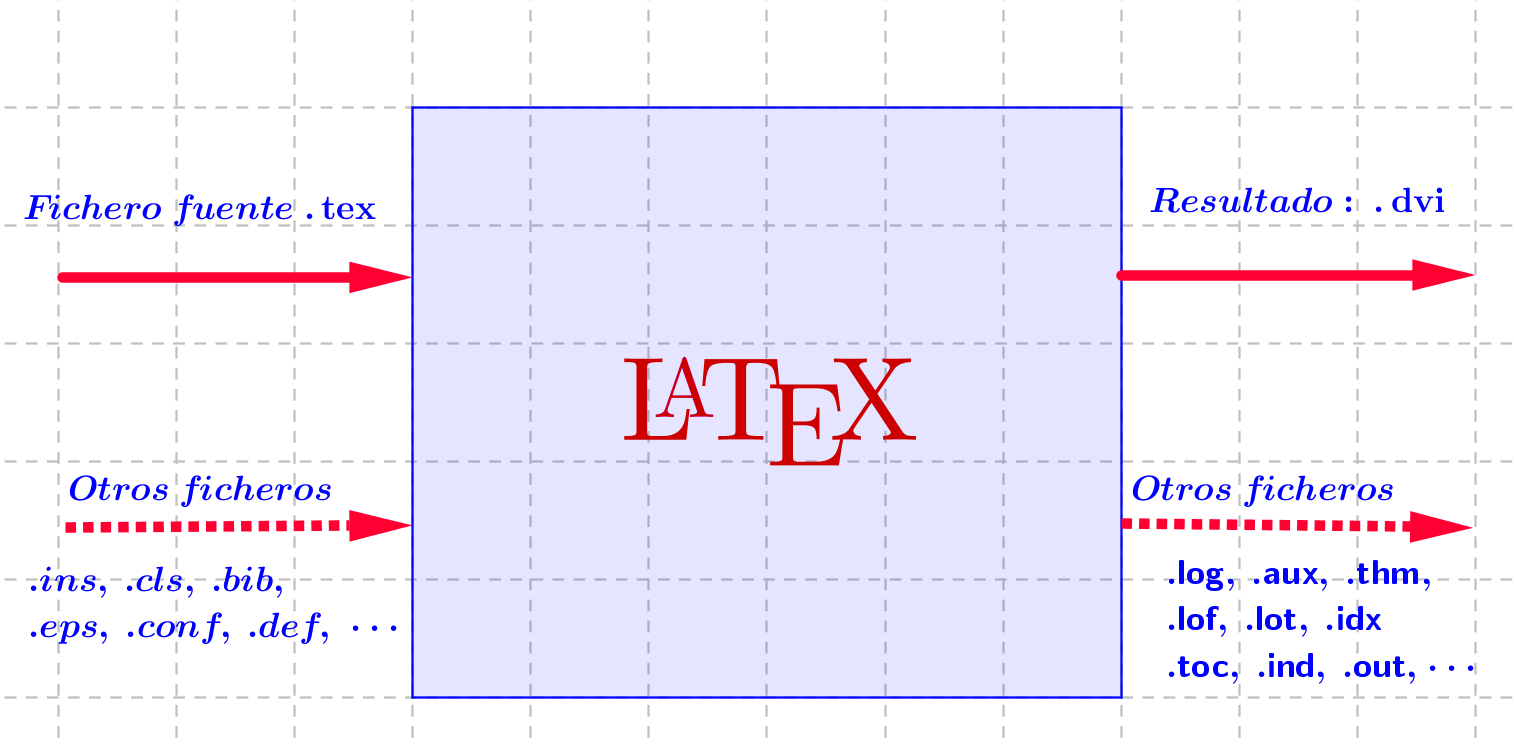
\includegraphics[scale=0.6]{diagrama.png}
\end{figure}

